documentclass
\documentclass[a4paper]{article}
\usepackage[utf8]{inputenc}
\usepackage[T1]{fontenc}
\usepackage{amsmath}
\usepackage{tikz}
\usetikzlibrary{arrows.meta}

\begin{document}

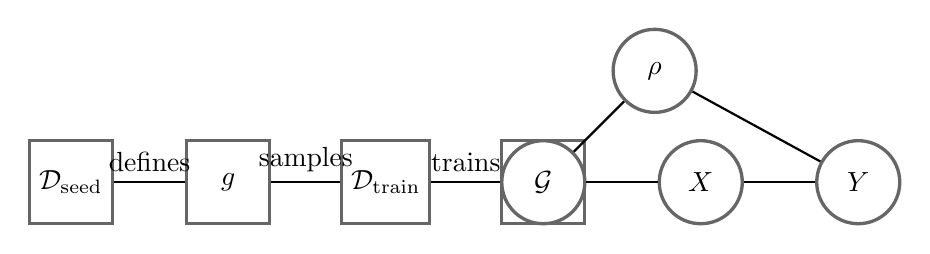
\begin{tikzpicture}[node distance=2cm, >=Latex]
    \tikzstyle{block} = [rectangle, draw=black!60, fill=white!5, very thick, minimum height=3em, minimum width=3em, align=center]
    \tikzstyle{arrow} = [thick,-]

    \node[block] (D_seed) {$\mathcal{D}_{\text{seed}}$};
    \node[block, right of=D_seed] (G) {$g$};
    \node[block, right of=G] (D_train) {$\mathcal{D}_{\text{train}}$};
    \node[block, right of=D_train] (W) {$w$};

    \draw[arrow] (D_seed) -- node[above] {defines} (G);
    \draw[arrow] (G) -- node[above] {samples} (D_train);
    \draw[arrow] (D_train) -- node[above] {trains} (W);
    
    \begin{scope}[xshift=6cm]
        \node[circle, draw=black!60, fill=white!5, very thick, minimum height=3em, minimum width=3em] (G) {$\mathcal{G}$};
        \node[circle, draw=black!60, fill=white!5, very thick, minimum height=3em, minimum width=3em, right of=G] (X) {$X$};
        \node[circle, draw=black!60, fill=white!5, very thick, minimum height=3em, minimum width=3em, above right of=G] (rho) {$\rho$};
        \node[circle, draw=black!60, fill=white!5, very thick, minimum height=3em, minimum width=3em, right of=X] (Y) {$Y$};

        \draw[arrow] (G) -- node[] {} (rho);
        \draw[arrow] (G) -- node[] {} (X);
        \draw[arrow] (rho) -- node[] {} (Y);
        \draw[arrow] (X) -- node[] {} (Y);
    \end{scope}
\end{tikzpicture}

\end{document}